\documentclass[11pt]{article}

\usepackage{amsmath,amssymb,amsfonts}
\usepackage{graphicx}
\usepackage{pgfplots}
\usepackage{multicol}
\usepackage{enumitem}

\setlength{\topmargin}{-.5in} \setlength{\textheight}{9.25in}
\setlength{\oddsidemargin}{0in} \setlength{\textwidth}{6.8in}


\begin{document}

\Large

\noindent{\bf Name: \hfill Date: \hfill Exam 2 \hfill Precalculus - Hargus}

\medskip\hrule
\vspace{20pt}

\noindent \textbf{Instructions:} Please \textbf{show all work} on the test paper (partial credit may be awarded for correct work, even if your answer is wrong). You may use the back side if you run out of room. Calculators are not allowed, but \textbf{simplify} your answers as much as you can. Cheating of any kind will result in a score of zero.

\vspace{10pt}

\begin{enumerate}

\item (8 points) Convert from radians to degrees or from degrees to radians.
\begin{multicols}{2}
\begin{enumerate}[itemsep=30pt]
    \item $\frac{\pi}{3}$
    \item $\frac{5\pi}{4}$
    \item $270^{\circ}$
    \item $120^{\circ}$
\end{enumerate}
\end{multicols}
\vspace{30pt}


\item (12 points) Evaluate the expression.
\begin{multicols}{2}
\begin{enumerate}[itemsep=60pt]
    \item $\log_{5}{125} = $
    \item $\log_{2}{\frac{1}{\sqrt[3]{16}}} = $
    \item $\log_{\pi}{\pi^5} = $
    \item $\sin{45^{\circ}} = $
    \item $\tan{\frac{2\pi}{3}} = $
    \item $\sec{\frac{3\pi}{2}} = $
\end{enumerate}
\end{multicols}
\vspace{60pt}


\item (5 points) Write an equation $f(t)$ for the number of movie tickets sold at Balijie Theater in year $t$. This year ($t=0$) there were 50000 tickets sold and the number of tickets sold \textbf{increases} by $\%10$ each year.
\begin{flushright}
$f(t) =$ \rule{4cm}{0.4pt}
\end{flushright}


\newpage


\item (6 points) Write an equation $f(x)$ for the following exponential graph.
\vspace{10pt}
\begin{center}
\begin{tikzpicture}
\begin{axis}[ xlabel={$x$}, ylabel={$y$}
  ,axis lines=middle
  ,samples=1000, grid, thick
  ,domain=-10:10
  ,restrict y to domain=-10:10
  ,axis equal
  ,legend pos=outer north east
  ,xmin=-3, xmax=7,
  ,ymin=-3, ymax=10
  ]
\addlegendentry{$f(x)$}
\addplot+[no marks] {3 * 2^(-x)};
\node[label={45:{$(0,3)$}},circle,fill,inner sep=2pt] at (axis cs:0,3) {};
\node[label={45:{$(2,0.75)$}},circle,fill,inner sep=2pt] at (axis cs:2,0.75) {};
\end{axis}
\end{tikzpicture}
\end{center}

\begin{flushright}
$f(x) =$ \rule{4cm}{0.4pt}
\end{flushright}


\item (8 points) Find the domain and the range of the function, and also state the equations for any vertical or horizontal asymptotes.
\begin{enumerate}[itemsep=60pt]
    \item $f(x) = \sin(x)+1$
    \item $f(x) = \ln(x)$
    \item $f(x) = -2^x$
\end{enumerate}
\vspace{60pt}


\item (5 points) A penny is $\frac{1}{100}$ of a dollar. How many orders of magnitude bigger is a ten dollar bill than a penny?
\vspace{20pt}


\newpage



\item (12 points) Solve for x.
\begin{multicols}{2}
\begin{enumerate}[itemsep=50pt]
    \item $\ln(x) = 5$
    \item $3\log_{2}(x) + 1 = 7$
    \item $e^{\ln(x)}=670$
    \item $\sin(x)=\frac{1}{2} \hspace{20pt} (\frac{\pi}{2} \leq x \leq \pi)$
\end{enumerate}
\end{multicols}
\vspace{50pt}


\item (8 points) Find the coordinates of the vertex for the following quadratic functions.
\begin{enumerate}[itemsep=40pt]
    \item $f(x) = 4(x-1)^2 + 8$
    \item $f(x) = x^2 - 2x + 6$ \\
\end{enumerate}
\vspace{100pt}

\item (6 points) Consider the function $f(x) = 2^x + 3$. True or false?
\begin{enumerate}[itemsep=20pt]
    \item \rule{1cm}{0.4pt} $f(x)$ has a horizontal asymptote at $y=3$.
    \item \rule{1cm}{0.4pt} $\displaystyle{\lim_{x \to \infty} f(x) = \infty}$
    \item \rule{1cm}{0.4pt} $\displaystyle{\lim_{x \to -\infty} f(x) = \infty}$
\end{enumerate}
\vspace{20pt}


\newpage

% \noindent{\bf Name: \hfill Date: \hfill Midterm 1 \hfill Precalculus - Hargus}

% \medskip\hrule
% \vspace{10pt}


\item (6 points) Use synthetic division to divide the following (Write your answer in \textbf{fraction form}).

\vspace{10pt}
$\displaystyle{\frac{x^3 - 5x^2 + 3x + 7}{x-3}} $
\vspace{100pt}

\item (6 points) Find the zeroes of the following functions. 
\begin{enumerate}[itemsep=10pt]
    \item $f(x) = x(x-1)^{3}(x-3)$
    \vspace{60pt}
    \begin{flushright}
    $x=$ \rule{4cm}{0.4pt}
    \end{flushright}
    
    \item $f(x) = x^2 + 3x + 1$
    \vspace{60pt}
    \begin{flushright}
    $x=$ \rule{4cm}{0.4pt}
    \end{flushright}
\end{enumerate}
\vspace{10pt}

\item (6 points) Sketch the graph of $f(x) = x(x-2)(x+2)$.
\vspace{10pt}
\begin{center}
\begin{tikzpicture}
\begin{axis}[ xlabel={$x$}, ylabel={$y$}
  ,axis lines=middle
  ,samples=1000, grid, thick
  ,domain=-10:10
  ,restrict y to domain=-10:10
  ,axis equal
  ,legend pos=outer north east
  ,xmin=-6, xmax=6,
  ,ymin=-5, ymax=5
  ];
% \addplot+[no marks] {(x+3)^2*(x-3)/20};
\end{axis}
\end{tikzpicture}
\end{center}


\newpage


\item (6 points) The graph of $f(x)=\sin(x)$ is below. Draw $g(x)=2\sin(2x)$.
\vspace{4pt}
\begin{center}
\begin{tikzpicture}
\begin{axis}[ xlabel={$x$}, ylabel={$y$}
  ,axis lines=middle
  ,samples=1000, grid, thick
  ,domain=-10:10
  ,restrict y to domain=-10:10
  ,legend pos=outer north east
  ,xmin=-6.4, xmax=6.4,
  ,ymin=-3, ymax=3
  , 
    xtick={
        -6.28318, -3.14159, 
        3.14159, 6.28318
    },
    xticklabels={
        $-2\pi$, $-\pi$, 
        $\pi$, $2\pi$
    }
    % xtick={
    %     -6.28318, -4.7123889, -3.14159, -1.5708,
    %     1.5708, 3.14159, 4.7123889, 6.28318
    % },
    % xticklabels={
    %     $-2\pi$, $-\frac{3\pi}{2}$, $-\pi\hspace{0.30cm}$, $-\frac{\pi}{2}$,
    %     $\frac{\pi}{2}$, $\pi\hspace{0.10cm}$, $\frac{3\pi}{2}$, $\hspace{0.25cm} 2\pi$
    % }
  ]
\addplot+[no marks] {sin(deg(x))};
\addlegendentry{$f(x)$}
\end{axis}
\end{tikzpicture}
\end{center}


\item (6 points) The graph of $f(x)$ is drawn below. Draw the graph of $f^{-1}(x)$.
\vspace{10pt}
\begin{center}
\begin{tikzpicture}
\begin{axis}[ xlabel={$x$}, ylabel={$y$}
  ,axis lines=middle
  ,samples=1000, grid, thick
  ,domain=-10:10
  ,restrict y to domain=-10:10
  ,axis equal
  ,legend pos=outer north east
  ,xmin=-5, xmax=5,
  ,ymin=-5, ymax=5
  ]
\addplot+[no marks] {e^x};
\addlegendentry{$f(x)$}
\end{axis}
\end{tikzpicture}
\end{center}


\vspace{10pt}
\item \textbf{Extra Credit} (5 points) Solve for x.
$$\frac{3^x - 3^{-x}}{2} = 5$$

\end{enumerate}

\end{document} 